
\chapter{Las teorías del comercio internacional y movimientos de los factores productivos}




\section{Ventajas absolutas en términos de precios unitarios o valor del trabajo}



\begin{ejercicio}

\textbf{Ventajas absolutas en términos de precios unitarios o valor del trabajo}

Supongamos un mundo con 2 países (N es nuestra nación y E el país extranjero), que producen dos bienes (X e Y). Para la producción de ambos bienes se utiliza tan sólo el factor trabajo ($L$). 

¿Le interesa el comercio internacional a ambos países? Para dar respuesta a este interrogante ha de cumplimentar las siguientes fases:

\begin{enumerate}
    \item Calcular los precios unitarios o valor del trabajo de la producción de $X$ e $Y$ y representarlos en una tabla, sabiendo que el precio unitario o valor trabajo ($v$) es el número de horas de trabajo ($L$), que es necesario para producir una unidad de un bien.
    \item Identificar para cada país, en qué producto es más eficiente y, por tanto, posee ventajas absolutas.
    \item Inferir, desde la ley de las ventajas absolutas, en qué se especializará cada país.
\end{enumerate}
\end{ejercicio}




\begin{solucion}[Práctica 2]

\end{solucion}

\subsection{Introducción Teórica: El Principio de la Ventaja Absoluta}

La teoría clásica del comercio, desarrollada inicialmente por Adam Smith, se fundamenta en el \textbf{principio de la ventaja absoluta}. Este principio establece que la especialización internacional y el comercio serán mutuamente beneficiosos cuando una nación tenga una \textbf{ventaja de coste absoluta} en la producción de un bien y la otra nación posea una ventaja de coste absoluta en el otro bien.

El coste se determina bajo la \textbf{teoría del valor del trabajo}, que asume que el trabajo ($L$) es el único factor de producción y que el coste o precio de un producto depende exclusivamente de la cantidad de trabajo requerida para fabricarlo. Una nación es considerada \textbf{absolutamente más eficiente} en la producción de un bien si utiliza menos trabajo para fabricar una unidad de producción.

Para que el mundo se beneficie de la especialización, cada nación debe tener un producto en el que sea más eficiente en su producción que su socio comercial. La nación que produce un bien a un coste menor debería especializarse en ese bien y exportarlo, mientras que importa el producto que fabrica a un coste mayor.

\subsection{Desarrollo de la Actividad Práctica}

Consideremos un mundo simplificado con dos países (Nación, N, y Extranjero, E) que producen dos bienes (X e Y) utilizando únicamente el factor trabajo ($L$).

\subsubsection*{Fase 1: Cálculo de los precios unitarios o valor del trabajo}

El \textbf{precio unitario o valor del trabajo} ($v$) de la producción de un bien se define como el número de horas de trabajo ($L$) necesarias para producir una unidad de dicho bien. Asumimos los siguientes requerimientos unitarios de trabajo ($a_{Li}$):

\begin{center}
\captionof{table}{Valor del Trabajo (Horas) Requerido por Unidad de Producto}
\begin{tabular}{|c|c|c|}
    \hline
    \textbf{Producto} & \textbf{Nación (N)} & \textbf{Extranjero (E)} \\
    \hline
    X & 4 & 10 \\
    \hline
    Y & 8 & 5 \\
    \hline
\end{tabular}
\end{center}

\begin{figure}[H]
    \centering
    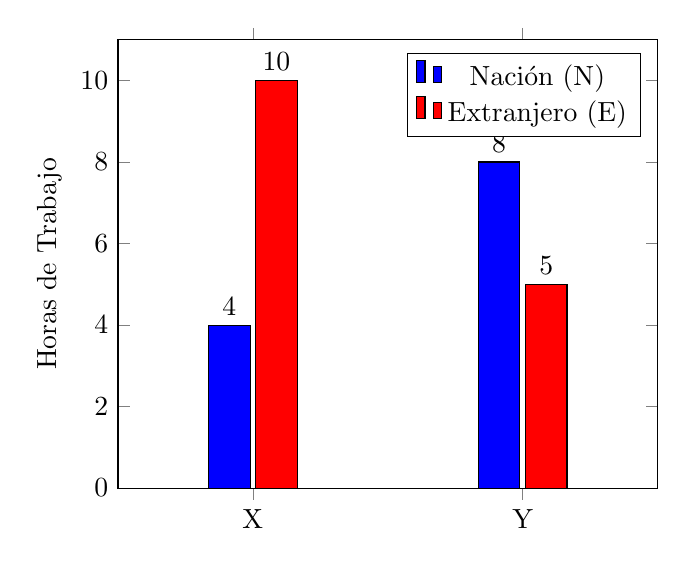
\begin{tikzpicture}
        \begin{axis}[
            symbolic x coords={X, Y},
            xtick=data,
            ylabel={Horas de Trabajo},
            legend pos=north east,
            bar width=15pt,
            ybar,
            ymin=0,
            nodes near coords,
            nodes near coords align={vertical},
            enlarge x limits=0.5
        ]
            \addplot[fill=blue] coordinates {(X, 4) (Y, 8)};
            \addplot[fill=red] coordinates {(X, 10) (Y, 5)};
            \legend{Nación (N), Extranjero (E)}
        \end{axis}
    \end{tikzpicture}
    \caption{Comparación de Horas de Trabajo Requeridas por Unidad de Producto}
    \label{fig:comparacion_horas_trabajo}
\end{figure}

\subsubsection*{Fase 2: Identificación de la Ventaja Absoluta}

Se compara el valor del trabajo requerido ($v$ o $a_{Li}$) para cada bien entre los dos países. El país que requiera menos horas de trabajo posee la ventaja absoluta.

\begin{enumerate}
    \item \textbf{Producción del Bien X:}
    \begin{itemize}
        \item Nación (N): 4 horas.
        \item Extranjero (E): 10 horas.
        \item Dado que $4 < 10$, la \textbf{Nación (N)} tiene ventaja absoluta en la producción del Bien X.
    \end{itemize}
    
    \item \textbf{Producción del Bien Y:}
    \begin{itemize}
        \item Nación (N): 8 horas.
        \item Extranjero (E): 5 horas.
        \item Dado que $5 < 8$, el \textbf{Extranjero (E)} tiene ventaja absoluta en la producción del Bien Y.
    \end{itemize}
\end{enumerate}

\subsubsection*{Fase 3: Especialización según la Ley de las Ventajas Absolutas}

De acuerdo con el principio de la ventaja absoluta, cada nación se beneficiará al especializarse en la producción de aquel producto que elabora a un coste menor que la otra nación.

\begin{itemize}
    \item La \textbf{Nación (N)} es más eficiente en la producción del Bien X y, por lo tanto, se \textbf{especializará en X} (y lo exportará).
    \item El \textbf{Extranjero (E)} es más eficiente en la producción del Bien Y y, por lo tanto, se \textbf{especializará en Y} (y lo exportará).
\end{itemize}

\subsection{Conclusión sobre el Interés del Comercio Internacional}

La pregunta inicial era: "¿Le interesa el comercio internacional a ambos países?".

\textbf{Sí, a ambos países les interesa el comercio internacional.}

Dado que la Nación (N) tiene ventaja absoluta en X y el Extranjero (E) tiene ventaja absoluta en Y, la especialización de cada país en el bien en el que es más productivo conduce a un \textbf{aumento en la producción mundial}. Al especializarse, el mundo utiliza sus recursos (en este caso, el factor trabajo) de forma más eficiente. El resultado es una producción conjunta más cuantiosa que se distribuye a las dos naciones a través del comercio, brindando una fuente de \textbf{ganancia mutua}.

Este ejemplo ilustra cómo el comercio es una actividad de suma positiva, donde ambas partes ganan al enfocarse en lo que relativamente hacen mejor.
